\section*{Assignment 3: Statistical Evaluation}
\subsection*{Assignment 2}
\subsubsection*{1. Fix and, if necessary, rerun your experiment according to the feedback in class.}
We were not suggested to re-run the experiment.

\subsubsection*{2. Compare the observed and commanded motions: do they fit? if not, describe possible causes for this.} \update{All readings up to significant digits.}

\begin{figure}[H]
\centering
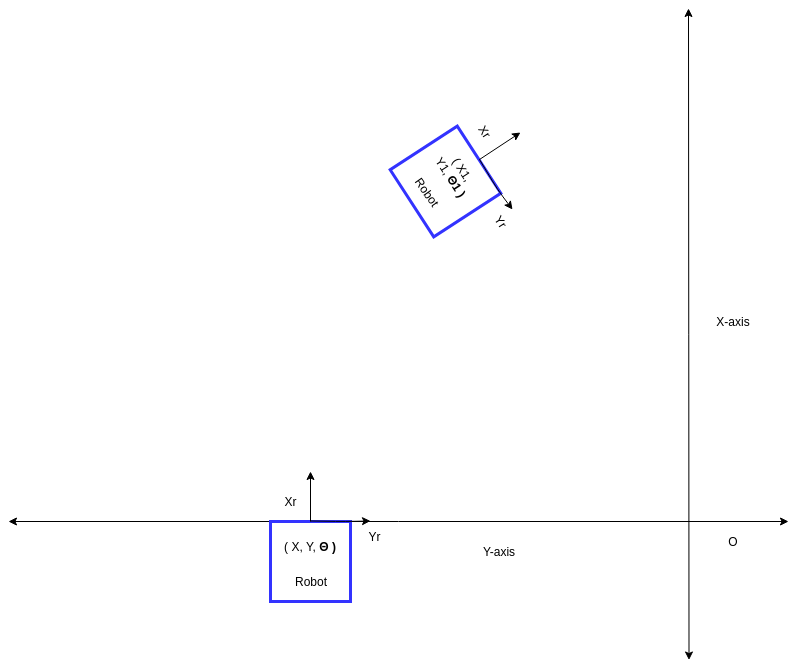
\includegraphics[width=0.5\textwidth]{exp_setup.png}
\caption{Schematic diagram for specifying conventions.}
\label{schematic-convention}
\end{figure}

Fig. \ref{schematic-convention} defines the signs and conventions used for following calculations. 
\begin{itemize}
	\item O : Origin of world co-ordinate frame
	\item Xr : X-axis of robot co-ordinate frame 
	\item Yr : X-axis of robot co-ordinate frame
	\item $\theta$ : Rotation of Xr around O in CCW direction
	\item (X, Y, $\theta$) :  Initial position and orientation of robot frame in world co-ordinate frame
	\item (X1, Y1, $\theta$1) : Final position and orientation of robot frame after the trail in world co-ordinate frame
\end{itemize}

\par On real robot, origin of robot co-ordinate frame coincides with the center of axle of the wheels. $Xr$ is perpendicular to the axle and points in the direction of robot's forward motion. \newline
\par Observing the geometrical structure, it is easy to conclude that position $(X, Y)$ of the robot is geometric mean of positions of wheels. 
\vspace{0.5cm}\\

\textbf{Parameters used in experiments}
\begin{itemize}
	\item commanded speed for wheel ($v$) = 18 cm/sec
	\item time ($t$) = 2250 milliseconds
	\item turn rate ($t_r$) = 40 ($t_r$ specifies the sharpness of the turn.)
	\item Ratio between inner and outer wheel speeds is given by,
	\begin{equation}
	r_{io} = \frac{100 - t_r}{100}
	\end{equation}
	\item The relation between inner and outer wheel speeds is given by,
	\begin{equation}
	v_i = t_r \cdot v_o
	\end{equation}
	where,
	\begin{itemize}
	\item linear speed of inner wheel ($v_i$) = $r_i * \omega$ cm/s.
	\item linear speed of outer wheel ($v_o$) = $(r_i + t_w ) * \omega$ cm/s.
	\end{itemize}
	\item Distance of center of robot axle from center of rotation ($r_i$) in cm 
	\item rotational speed of center of the axle of wheels = $\omega$ rad/s.
	\item distance between wheels (track width $t_w$) = 11.4 cm 
	\item initial position of right wheel ($X_{ri}$, $Y_{ri}$) = (0.0 cm, 20.6 cm) 
	\item initial position of left wheel ($X_{le}$, $Y_{le}$) = (0.0 cm, 35.1 cm)
	\item initial pose of robot (X, Y, $\theta$) = (0.0 cm, 27.85 cm, 0.0 rad)
\end{itemize}

\textbf{Systematic error}\\
\begin{itemize}
\item The error in wheel diameter can be defined as ratio between two wheel diameters defined in Eq. \ref{wheel-error},
\begin{equation}
E_D = \frac{D_R}{D_L} = 1.0
\end{equation}

\item The error in wheelbase is computed from Eq. \ref{track-width-error},
\begin{equation}
E_B = \frac{b_{\text{actual}}}{b_{\text{assumed}}} = \frac{11.4}{18.6} = 0.78
\end{equation}
\end{itemize}
\textbf{Analytical derivations}
\par Angular pose of the robot ($\theta$) can be calculated using individual wheel positions with help of following formula:
\begin{equation}
\theta = \left[ tan^{-1}\left(\frac{Y_{ri} - Y_{le}}{X_{ri} - X_{le}}\right) - \frac{\pi}{2} \right] \cdot \frac{180}{\pi} \qquad\qquad \text{(in degrees)}
\label{theta-orientation}
\end{equation}
For right and left turn motion, we compute the angular pose as follows:
\begin{equation}
\theta_r/ \theta_l = \cos^{-1}\left(\frac{2r^2 - s^2}{r^2}\right)
\label{lr-ang-pose}
\end{equation}
where $s$ is straight-line displacement between the initial and final pose and $r$ is radius of the circle on which the robot traverses (refer to Eq. \ref{radius-circle}).
\begin{enumerate}
\item \textbf{Straight motion}

	\textbf{Commanded Motion}

	\begin{itemize}

		\item expected distance to be traveled by by both wheels in y-axis direction = $0$ cm
	
		\item expected position of right wheel ($X_{ri}$, $Y_{ri}$) = (0.0 + $v\cdot t$, 20.6 cm) \\
			   = (0.0 + 40.5 cm, 20.6 cm)\\
			 = (40.5 cm, 20.6 cm)
	
		\item expected position of left wheel ($X_{le}$, $Y_{le}$) = (0.0 + $v\cdot t$, 35.1 cm) \\
		= (0.0 + 40.5 cm, 35.1 cm)\\
		= (40.5 cm, 35.1 cm)
	
		\item expected position of robot $(X, Y, \theta) = (0.0 + 40.5 \text{ cm}, 27.85 \text{ cm}, 0.0^{\circ}) = (40.5 \text{ cm}, 27.85 \text{ cm}, 0.0^{\circ})$
\end{itemize}
	
\textbf{Observed motion}:
\begin{itemize}
\item mean distance traveled by right wheel in x-direction = 40.5 cm
\item mean distance traveled by left wheel in x-direction = 40.3 cm 
\item mean distance traveled by right wheel in y-direction = 0.1 cm 
\item mean distance traveled by left wheel in y-direction = 0.1 cm 
\end{itemize}

The observed final pose is given as,
\begin{equation}
\begin{array}{rcl}
x_r &=& 40.4 \text{ cm} \\
y_r &=& 27.9 \text{ cm} \\
\theta_r &=& tan^{-1}\cfrac{Y_{ri} - Y_{le}}{X_{ri} - X_{le}} - 0.5\cdot{\pi} = 0.6^{\circ} \qquad \text{(Using Eq. \ref{theta-orientation})}
\end{array}
\end{equation}
	
\item \textbf{Right Turn} \\
	\textbf{Expected motion}
	\newline
	The radius of the circle is given by,
	\begin{equation}
	r_i = \cfrac{\cfrac{(100 - t_r)\cdot t_{w}}{100}}{2 \cdot \cfrac{t_{r}}{100}} = 22.8 \text{ cm}
	\label{radius-circle}
	\end{equation}
	
	The angular velocity is computed as follows:
	\begin{equation}
	\omega = \cfrac{r_i \cdot \cfrac{t_r}{100}}{t_w} = \frac{18}{22.8} = 0.79 \text{ rad/sec}
	\end{equation}
	
	The final pose is computed as,
	\begin{equation}
	\begin{array}{rcl}
	x_r &=& r_{i}\cdot sin(\omega * t) - 4.8 \text{ cm} = 17.5 \text{ cm}\\
	y_r &=& r_{i}\cdot sin(\omega * t) + 5.05 \text{ cm} = 0.5 \text{ cm} \\
	\theta_r &=& 90.7^{\circ} \hspace{5cm} \text{(Using Eq. \ref{lr-ang-pose})}
	\end{array}
	\end{equation}
	
	
	\textbf{Observed motion}
	\begin{equation}
	\begin{array}{rcl}
	x_{r} &=& 17.8 \text{ cm} \\
	y_{r} &=& 2.8 \text{ cm} \\
	\theta_r &=& 89.8^{\circ} \hspace{5cm} \text{(Using Eq. \ref{lr-ang-pose})}
	\end{array}
	\end{equation}
	
	\item \textbf{Left Turn} \\
	
	\textbf{Expected motion}
	
	The left turn motion is mirrored motion that of right turn about the line passing robot's initial position and parallel to x-axis. 
	hence,
	
	The final pose is computed as,
	\begin{equation}
	\begin{array}{rcl}
	x_r &=& r_{i}\cdot sin(\omega * t) - 4.8 \text{ cm} = 17.5 \text{ cm}\\
	y_r &=& 50.15 - r_{i}\cdot sin(\omega * t) \text{ cm} = 50.15 - (-4.7) = 54.8 \text{ cm} \\
	\theta_r &=& 84.5^{\circ} \hspace{5cm} \text{(Using Eq. \ref{lr-ang-pose})}
	\end{array}
	\end{equation}
	
	\textbf{Observed motion}
	\begin{equation}
	\begin{array}{rcl}
	x_{l} &=& 17.8 \text{ cm} \\
	y_{l} &=& 52.9 \text{ cm} \\
	\theta_r &=& 84.5^{\circ} \hspace{5cm} \text{(Using Eq. \ref{lr-ang-pose})}
	\end{array}
	\end{equation}
	
	
\end{enumerate}

In case of straight line motion, the commanded motion matches with the observed motion. Small random error can be observed in the readings but it can be the result of inaccurate placement of robot before starting the run, inaccurate measurement or LED displacement. 

In case of turning motion, a large error can be observed. The facts for formula derivation for calculation of motion are taken from API provided by lejos library (\href{http://www.lejos.org/nxt/nxj/api/lejos/robotics/navigation/DifferentialPilot.html#steer(double)}{link}\footnote{http://www.lejos.org/nxt/nxj/api/lejos/robotics/navigation/DifferentialPilot.html$\#$steer(double)}). This API documentation does not clarify the effect of turn rate used in \textit{steer} function well enough. The absolute speed value of outer wheel is not clarified. Hence it is assumed to be equal to absolute speed set by DifferentialPilot. This can be the cause of error.
Another reason of error can be the value of track width parsed in the code which is 18.6 cm but it is 14.5 cm on real robot.
If the formula provided in the documentation of lejos API for calculating speed of each wheel set by steer function considers outer wheel's speed equal to absolute speed set by DifferentialPilot function, then the error in track width value must not have any effect on experiment. But clearly, this is not the fact, the assumptions made on turn speed and steer function are needed to be revisited and made cleared with some other sources.      

\newpage
\subsubsection*{3. Fit a Gaussian to your data and judge if the data is truly Gaussian or if it follows another distribution.}

\begin{figure}[ht]
\centering
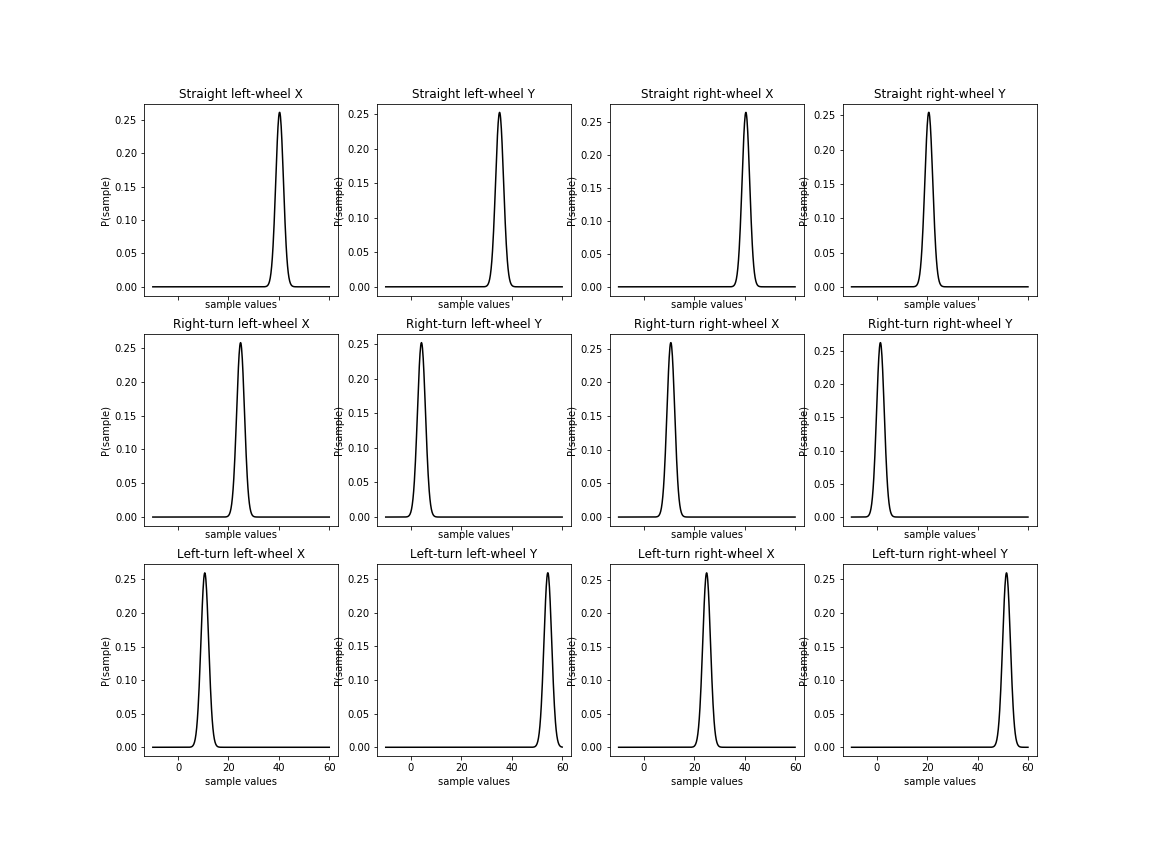
\includegraphics[width=\textwidth]{gaussian_fits.png}
\caption{Gaussian fit for the data using scikit-learn KernelDensity function. \update{x labels with units.}}
\label{gaussian}
\end{figure}


\begin{figure}[H]
\centering
\begin{subfigure}[b]{0.3\textwidth}
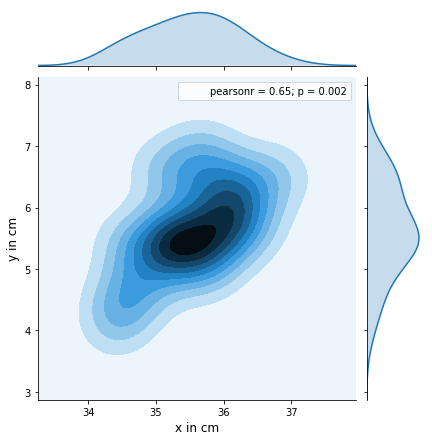
\includegraphics[width=\textwidth]{right_motion_distribution.png}
\caption{Right turn final pose.}
\label{distribution-right-turn}
\end{subfigure}
\qquad
\begin{subfigure}[b]{0.3\textwidth}
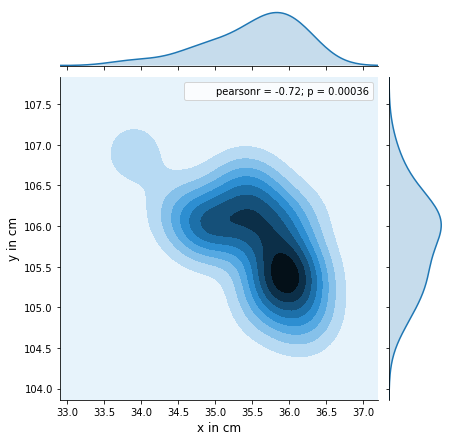
\includegraphics[width=\textwidth]{left_motion_distribution.png}
\caption{Left turn final pose.}
\label{distribution-right-turn}
\end{subfigure}
\qquad
\begin{subfigure}[b]{0.3\textwidth}
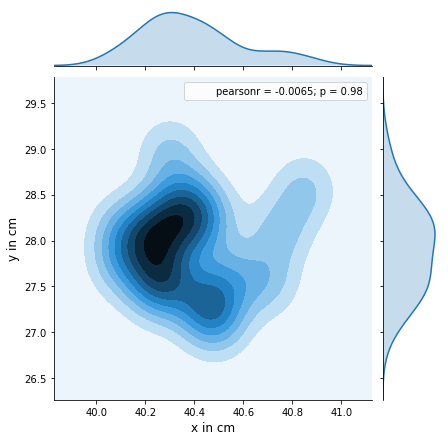
\includegraphics[width=\textwidth]{straight_motion_distribution.png}
\caption{Straight motion final pose.}
\label{distribution-straight-motion}
\end{subfigure}
\caption{Gaussian and marginal distributions \update{Final pose distribution.}}
\end{figure}

\newpage
\subsubsection*{4. Compare the estimated uncertainty of the measurement process itself with the statistical uncertainty of the observed end poses.}

\begin{table}[H]
	\centering
	\begin{tabular}{| l | c | c | c | c | c | c |}
		\hline
		& \multicolumn{2}{c|}{left-turn motion} & \multicolumn{2}{c|}{ right-turn motion} & \multicolumn{2}{c|}{straight motion} \\
		\hline
		& right wheel & left wheel & right wheel & left wheel & right wheel & left wheel \\
		\hline
		Mean linear deviation $(\delta x, \delta y)$ cm & (0.1, 0.9) & (0.6, 0.8)
		& (0.7, 0.9) & (0.2, 0.9) & (0.5, 0.4) & 0.3, 0.4) \\
		\hline
		Mean ang. deviation ($\delta \theta$) degrees & 0.9 & 2.3 & 2.7 & 1.1 & 0.6 & 0.6 \\
		\hline
		$\sigma$ in final pose: $(\sigma_x, \sigma_y)$ cm & (0.3, 0.3) & (0.3, 0.3) & (0.3, 0.2) & (0.4, 0.5) & (0.2, 0.5) & (0.3, 0.5)\\
		\hline
		uncertainty in pose $(\delta x \pm \sigma_x)$ cm & $(0.1 \pm 0.3)$ & $(0.6 \pm 0.3)$ & $(0.7 \pm 0.3)$ & $(0.2 \pm 0.4)$ & $(0.5 \pm 0.2)$ & $(0.3 \pm 0.3)$ \\
		uncertainty in pose $(\delta y \pm \sigma_y)$ cm & $(0.9 \pm 0.3)$ & $(0.8 \pm 0.3)$ & $(0.9 \pm 0.2)$ & $(0.9 \pm 0.5)$ & $(0.4 \pm 0.5)$ & $(0.2 \pm 0.5)$ \\
		\hline
	\end{tabular}
	\caption{Statistical summary of observed robot motion. Refer to Eq. \ref{mean-deviation}, \ref{standard-deviation}, \ref{mean-angular-deviation}. \update{Measurement uncertainty}}
	\label{stats}
\end{table}
There are three type of uncertainties which we estimated which can occur in the measurement. 
\begin{enumerate}
	\item Uncertainty in initial linear position of robot
	\item Uncertainty in initial angular position of robot
	\item uncertainty in measuring co-ordinates of the wheels
\end{enumerate}   

$1^{st}$ uncertainty will cause small linear error in measurement of wheel position equivalent to error in initial linear position.

$2^{nd}$ uncertainty will cause huge error in measurement of wheel position which will increase with distance travelled by robot. 

$3^{rd}$ uncertainty will cause small error (1 - 2 mm) in linear position of wheels.

\sectionLine
\subsection*{Deliverables 2}
Update your previous week’s report and add a description of the test for a match with a Gaussian distribution as well as a description of the observed differences between the observed and the computed motion and the actual and expected accuracy and precision. Include appropriate figures, diagrams, and images backing up any claims you make. The report must be self-contained and provide enough details to support any statement you make. If applicable, include a section on problems encountered. Your update should cover:

\subsubsection*{1. Any possible pre-processing of your data, like outlier detection and removal.}
We did not require any outlier detection algorithm since the data collection did not contain any outliers.

\subsubsection*{2. Fit of a Gaussian, either two individual ones in the x and y directions for each of the three cases or a proper two-dimensional distribution per case.}
We were able to fit the Gaussian to the data as shown in fig. \ref{gaussian}.

\subsubsection*{3. Check whether the data are actually distributed according to a Gaussian distribution.}
The data is too limited to conclude whether it comes from Gaussian distribution, however we were able to fit the data to a Gaussian distribution.

\subsubsection*{4. List of used software, including source of any function you wrote for performing your analysis.}
The software code is attached with the report.

\subsubsection*{5. An answer to the following question: When analysing the data with respect to the executed motions, which characteristic of the data do you establish here: the accuracy, the precision, or both?}

Because of the offset in the analytical calculations and actual mean of the readings, we can say that the executed motion was not accurate. But executed motion shows repeatability with lower variance, hence it can be concluded that the motion was precise. We will be revisiting our calculations by clearing the facts related to parameters used in the code, experiment will be re-performed if needed. In conclusion, with current calculations, turning motion was not accurate but it was precise. 
%%%%%%%%%%%%%%%%%%%%%%%%%%%%%%%%%%%%%%%%%%%%%%%%%%%%%%%%%%%%%%%%%%%%%%%%%%%%%